%\centering
%\scalebox{0.8}{
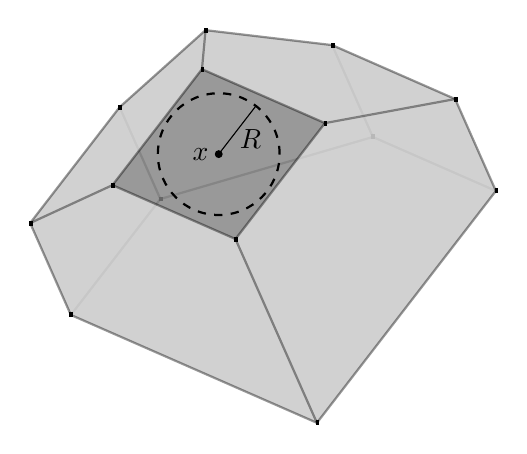
\begin{tikzpicture}
        [x={(0.258520cm, -0.583496cm)},
        y={(0.781193cm, -0.342529cm)},
        z={(-0.568247cm, -0.736347cm)},
        scale=2.000000,
        back/.style={loosely dotted, thin},
        edge/.style={color=black, thick, opacity=0.4},
        circle/.style={color=black, thick, dashed},
        facet/.style={fill=black!20,color=black!20,fill opacity=0.9},
        specialFacet/.style={fill=black!30,color=black!50,fill opacity=0.8},
        vertex/.style={inner sep=0.5pt,circle,draw=black!25!black,fill=black!75!black,thick,anchor=base},
        vertexC/.style={inner sep=5pt,circle,draw=black!100!black,fill=black!100!black,thick,anchor=base}]
%
%
%% Coordinate of the vertices:
%%

\coordinate (0.5, 0.5, -1.05) at (0.5, 0.5, 1.05);

\coordinate (-0.500, -0.500, -0.500) at (-0.500, -0.500, -0.500);
\coordinate (-1.00, 0.000, 0.000) at (-1.00, 0.000, 0.000);
\coordinate (-1.00, 0.000, 1.00) at (-1.00, 0.000, 1.00);
\coordinate (-1.00, 1.00, 0.000) at (-1.00, 1.00, 0.000);
\coordinate (-1.00, 1.00, 1.00) at (-1.00, 1.00, 1.00);
\coordinate (0.000, -1.00, 0.000) at (0.000, -1.00, 0.000);
\coordinate (0.000, -1.00, 1.00) at (0.000, -1.00, 1.00);
\coordinate (0.000, 0.000, -1.00) at (0.000, 0.000, -1.00);
\coordinate (0.000, 1.00, -1.00) at (0.000, 1.00, -1.00);
\coordinate (1.00, -1.00, 0.000) at (1.00, -1.00, 0.000);
\coordinate (1.00, -1.00, 1.00) at (1.00, -1.00, 1.00);
\coordinate (1.00, 0.000, -1.00) at (1.00, 0.000, -1.00);
\coordinate (1.00, 1.00, -1.00) at (1.00, 1.00, -1.00);
\coordinate (1.00, 1.00, 1.00) at (1.00, 1.00, 1.00);
%%
%%
%% Drawing edges in the back
%%
%%
%%
%% Drawing vertices in the back
%%
\node[vertex] at (1.00, -1.00, 0.000)     {};
\node[vertex] at (1.00, 0.000, -1.00)     {};
%%
%%
%% Drawing the facets
%%
\draw[edge] (0.000, -1.00, 0.000) -- (1.00, -1.00, 0.000);
\draw[edge] (0.000, 0.000, -1.00) -- (1.00, 0.000, -1.00);
\draw[edge] (1.00, 0.000, -1.00) -- (1.00, 1.00, -1.00);
\draw[edge] (1.00, -1.00, 0.000) -- (1.00, -1.00, 1.00);
\draw[edge] (1.00, -1.00, 0.000) -- (1.00, 0.000, -1.00);

\fill[facet] (1.00, 1.00, 1.00) -- (-1.00, 1.00, 1.00) -- (-1.00, 1.00, 0.000) -- (0.000, 1.00, -1.00) -- (1.00, 1.00, -1.00) -- cycle {};
\fill[facet] (1.00, 1.00, 1.00) -- (-1.00, 1.00, 1.00) -- (-1.00, 0.000, 1.00) -- (0.000, -1.00, 1.00) -- (1.00, -1.00, 1.00) -- cycle {};
\fill[facet] (0.000, -1.00, 1.00) -- (-1.00, 0.000, 1.00) -- (-1.00, 0.000, 0.000) -- (-0.500, -0.500, -0.500) -- (0.000, -1.00, 0.000) -- cycle {};
\fill[facet] (0.000, 1.00, -1.00) -- (-1.00, 1.00, 0.000) -- (-1.00, 0.000, 0.000) -- (-0.500, -0.500, -0.500) -- (0.000, 0.000, -1.00) -- cycle {};
\fill[specialFacet] (-1.00, 1.00, 1.00) -- (-1.00, 0.000, 1.00) -- (-1.00, 0.000, 0.000) -- (-1.00, 1.00, 0.000) -- cycle {};
\draw[edge] (1.00, -1.00, 1.00) -- (1.00, 1.00, 1.00);
\draw[edge] (1.00, 1.00, -1.00) -- (1.00, 1.00, 1.00);
\draw[edge] (0.000, -1.00, 1.00) -- (1.00, -1.00, 1.00);
\draw[edge] (0.000, 0.000, -1.00) -- (0.000, 1.00, -1.00);
\draw[edge] (0.000, 1.00, -1.00) -- (1.00, 1.00, -1.00);
%%
%%
%% Drawing edges in the front
%%
\draw[edge] (-0.500, -0.500, -0.500) -- (-1.00, 0.000, 0.000);
\draw[edge] (-0.500, -0.500, -0.500) -- (0.000, -1.00, 0.000);
\draw[edge] (-0.500, -0.500, -0.500) -- (0.000, 0.000, -1.00);
\draw[edge] (-1.00, 0.000, 0.000) -- (-1.00, 0.000, 1.00);
\draw[edge] (-1.00, 0.000, 0.000) -- (-1.00, 1.00, 0.000);
\draw[edge] (-1.00, 0.000, 1.00) -- (-1.00, 1.00, 1.00);
\draw[edge] (-1.00, 0.000, 1.00) -- (0.000, -1.00, 1.00);
\draw[edge] (-1.00, 1.00, 0.000) -- (-1.00, 1.00, 1.00);
\draw[edge] (-1.00, 1.00, 0.000) -- (0.000, 1.00, -1.00);
\draw[edge] (-1.00, 1.00, 1.00) -- (1.00, 1.00, 1.00);
\draw[edge] (0.000, -1.00, 0.000) -- (0.000, -1.00, 1.00);
%%
%%
%% Drawing the vertices in the front
%%
\node[vertex] at (-0.500, -0.500, -0.500)     {};
\node[vertex] at (-1.00, 0.000, 0.000)     {};
\node[vertex] at (-1.00, 0.000, 1.00)     {};
\node[vertex] at (-1.00, 1.00, 0.000)     {};
\node[vertex] at (-1.00, 1.00, 1.00)     {};
\node[vertex] at (0.000, -1.00, 0.000)     {};
\node[vertex] at (0.000, -1.00, 1.00)     {};
\node[vertex] at (0.000, 0.000, -1.00)     {};
\node[vertex] at (0.000, 1.00, -1.00)     {};
\node[vertex] at (1.00, -1.00, 1.00)     {};
\node[vertex] at (1.00, 1.00, -1.00)     {};
\node[vertex] at (1.00, 1.00, 1.00)     {};
%%

\draw[fill=black,color=black] (-1.00, 0.500, 0.50) -- (-1.0,0.5,0.08) node[pos=0.3,right]{$R$};
\draw[thick,fill=black,color=black] (-1.00, 0.500, 0.500) circle (0.5pt) node[left] {$x$};
\draw[circle] (-1.00, 0.50, 0.50) circle (11pt);

\end{tikzpicture}
%}
%\caption{A polytope in $\R^3$ (light gray) and a surface element (dark gray)}
%\end{figure}

